\documentclass[11pt,a4paper]{article}
\usepackage[T1]{fontenc}
\usepackage{lmodern}
\usepackage[margin=2.5cm]{geometry}
\usepackage{amsmath,amssymb,booktabs,graphicx,xcolor,multirow,array}
\usepackage{mathptmx}
\usepackage[authoryear,round]{natbib}
\usepackage{tikz}\usetikzlibrary{arrows.meta,positioning,shapes.geometric}
\usepackage{algorithm,algorithmic,capt-of,enumitem}
\usetikzlibrary{arrows.meta,positioning,shapes.geometric}

\newcommand{\btheta}{\boldsymbol{\theta}}
\newcommand{\bphi}{\boldsymbol{\phi}}
\newcommand{\bpsi}{\boldsymbol{\psi}}
\newcommand{\yobs}{\mathbf{y}_{\mathrm{obs}}}
\newcommand{\Real}{\mathbb{R}}
\usepackage[hidelinks]{hyperref}
% Values awaiting the final runs
\newcommand{\TBD}[1]{\textcolor{red}{\textbf{[#1]}}}
\renewcommand{\thetable}{S\arabic{table}}
\renewcommand{\thealgorithm}{S\arabic{algorithm}}
\renewcommand{\theequation}{S\arabic{equation}}
\renewcommand{\thefigure}{S\arabic{figure}}
\renewcommand{\thesection}{S\arabic{section}}

\title{Supplementary Material\\[4pt]
\large \textcolor{red}{[final EML title]}}
\author{K.~Nishioka, F.~Klempt, H.~Geisler, R.~Mukherjee, N.~Heine, K.~Doll-Nikutta,\\ M.~Stiesch, S.~P.~Szafra\'{n}ski, M.~Soleimani, P.~Junker}
\date{}

% generated by tools/fill_manuscript.py
\newcommand{\numRmseRangePhaseTwo}{\TBD{}}
\newcommand{\numRmseCS}{\TBD{}}
\newcommand{\numMapPgPgCS}{\TBD{}}
\newcommand{\numQloPgPgCS}{\TBD{}}
\newcommand{\numQhiPgPgCS}{\TBD{}}
\newcommand{\numQmedPgPgCS}{\TBD{}}
\newcommand{\numMapFnPgCS}{\TBD{}}
\newcommand{\numQloFnPgCS}{\TBD{}}
\newcommand{\numQhiFnPgCS}{\TBD{}}
\newcommand{\numQmedFnPgCS}{\TBD{}}
\newcommand{\numMapFnFnCS}{\TBD{}}
\newcommand{\numQloFnFnCS}{\TBD{}}
\newcommand{\numQhiFnFnCS}{\TBD{}}
\newcommand{\numQmedFnFnCS}{\TBD{}}
\newcommand{\numMapSoAnCS}{\TBD{}}
\newcommand{\numQloSoAnCS}{\TBD{}}
\newcommand{\numQhiSoAnCS}{\TBD{}}
\newcommand{\numQmedSoAnCS}{\TBD{}}
\newcommand{\numMapSoVeiCS}{\TBD{}}
\newcommand{\numQloSoVeiCS}{\TBD{}}
\newcommand{\numQhiSoVeiCS}{\TBD{}}
\newcommand{\numQmedSoVeiCS}{\TBD{}}
\newcommand{\numPhaseRCS}{\TBD{}}
\newcommand{\numRmseCH}{\TBD{}}
\newcommand{\numMapPgPgCH}{\TBD{}}
\newcommand{\numQloPgPgCH}{\TBD{}}
\newcommand{\numQhiPgPgCH}{\TBD{}}
\newcommand{\numQmedPgPgCH}{\TBD{}}
\newcommand{\numMapFnPgCH}{\TBD{}}
\newcommand{\numQloFnPgCH}{\TBD{}}
\newcommand{\numQhiFnPgCH}{\TBD{}}
\newcommand{\numQmedFnPgCH}{\TBD{}}
\newcommand{\numMapFnFnCH}{\TBD{}}
\newcommand{\numQloFnFnCH}{\TBD{}}
\newcommand{\numQhiFnFnCH}{\TBD{}}
\newcommand{\numQmedFnFnCH}{\TBD{}}
\newcommand{\numMapSoAnCH}{\TBD{}}
\newcommand{\numQloSoAnCH}{\TBD{}}
\newcommand{\numQhiSoAnCH}{\TBD{}}
\newcommand{\numQmedSoAnCH}{\TBD{}}
\newcommand{\numMapSoVeiCH}{\TBD{}}
\newcommand{\numQloSoVeiCH}{\TBD{}}
\newcommand{\numQhiSoVeiCH}{\TBD{}}
\newcommand{\numQmedSoVeiCH}{\TBD{}}
\newcommand{\numPhaseRCH}{\TBD{}}
\newcommand{\numRmseDS}{\TBD{}}
\newcommand{\numMapPgPgDS}{\TBD{}}
\newcommand{\numQloPgPgDS}{\TBD{}}
\newcommand{\numQhiPgPgDS}{\TBD{}}
\newcommand{\numQmedPgPgDS}{\TBD{}}
\newcommand{\numMapFnPgDS}{\TBD{}}
\newcommand{\numQloFnPgDS}{\TBD{}}
\newcommand{\numQhiFnPgDS}{\TBD{}}
\newcommand{\numQmedFnPgDS}{\TBD{}}
\newcommand{\numMapFnFnDS}{\TBD{}}
\newcommand{\numQloFnFnDS}{\TBD{}}
\newcommand{\numQhiFnFnDS}{\TBD{}}
\newcommand{\numQmedFnFnDS}{\TBD{}}
\newcommand{\numMapSoAnDS}{\TBD{}}
\newcommand{\numQloSoAnDS}{\TBD{}}
\newcommand{\numQhiSoAnDS}{\TBD{}}
\newcommand{\numQmedSoAnDS}{\TBD{}}
\newcommand{\numMapSoVeiDS}{\TBD{}}
\newcommand{\numQloSoVeiDS}{\TBD{}}
\newcommand{\numQhiSoVeiDS}{\TBD{}}
\newcommand{\numQmedSoVeiDS}{\TBD{}}
\newcommand{\numPhaseRDS}{\TBD{}}
\newcommand{\numRmseDH}{\TBD{}}
\newcommand{\numMapPgPgDH}{\TBD{}}
\newcommand{\numQloPgPgDH}{\TBD{}}
\newcommand{\numQhiPgPgDH}{\TBD{}}
\newcommand{\numQmedPgPgDH}{\TBD{}}
\newcommand{\numMapFnPgDH}{\TBD{}}
\newcommand{\numQloFnPgDH}{\TBD{}}
\newcommand{\numQhiFnPgDH}{\TBD{}}
\newcommand{\numQmedFnPgDH}{\TBD{}}
\newcommand{\numMapFnFnDH}{\TBD{}}
\newcommand{\numQloFnFnDH}{\TBD{}}
\newcommand{\numQhiFnFnDH}{\TBD{}}
\newcommand{\numQmedFnFnDH}{\TBD{}}
\newcommand{\numMapSoAnDH}{\TBD{}}
\newcommand{\numQloSoAnDH}{\TBD{}}
\newcommand{\numQhiSoAnDH}{\TBD{}}
\newcommand{\numQmedSoAnDH}{\TBD{}}
\newcommand{\numMapSoVeiDH}{\TBD{}}
\newcommand{\numQloSoVeiDH}{\TBD{}}
\newcommand{\numQhiSoVeiDH}{\TBD{}}
\newcommand{\numQmedSoVeiDH}{\TBD{}}
\newcommand{\numPhaseRDH}{\TBD{}}
\newcommand{\numPhaseRCommensalRange}{\TBD{}}
\newcommand{\numViabRmseRange}{\TBD{}}
\newcommand{\numAcceptRange}{\TBD{}}
\newcommand{\numSurgeBase}{\TBD{99--100}}
\newcommand{\numSurgeNoFn}{\TBD{10--13}}
\newcommand{\numSurgeAzero}{\TBD{2--6}}
\newcommand{\numProbSuppressed}{\TBD{0.87--0.90}}
\newcommand{\numUltHoursPerCond}{\TBD{}}
\newcommand{\numUltHoursAll}{\TBD{h}}
\newcommand{\numUltGpu}{\TBD{model}}
\newcommand{\numPhRtwo}{\TBD{0.78}}
\newcommand{\numPhRmse}{\TBD{0.13}}
\newcommand{\numPhNsamples}{\TBD{500}}
\newcommand{\numPhNpoints}{\TBD{12}}
\newcommand{\numGingipainR}{\TBD{0.90}}
\newcommand{\numZenodoDoi}{\TBD{DOI}}
\newcommand{\numTimingRows}{\quad Per condition & \TBD{h}$^\dagger$ & \TBD{h} & \TBD{x}\\
\quad All 4 cond.   & \TBD{h}$^\dagger$ & \TBD{h} & \TBD{x}\\}

\begin{document}
\maketitle

\section{Model derivation}
\label{sec:S_model}

\subsection*{State variables and kinematics}

Following \citet{Klempt2025ContinuumBiofilm, Klempt2024ContinuumGrowth}, the biofilm is described at a material point by two sets of internal variables: the volume fraction $\phi_i \in [0,1]$ occupied by species~$i$ ($i=1,\dots,n$; here $n=5$), and the viability fraction $\psi_i \in [0,1]$ representing the proportion of living cells within species~$i$.
The living volume fraction is then
\begin{equation}
\bar{\phi}_i := \phi_i\,\psi_i,
\qquad i=1,\dots,n.
\label{eq:living}
\end{equation}
An additional void fraction~$\phi_0$ closes the system via the holonomic constraint
\begin{equation}
\sum_{l=0}^{n}\phi_l(t) - 1 = 0 \quad\forall\,t.
\label{eq:constraint}
\end{equation}



\subsection*{Variational formulation}
The evolution equations are derived from the principle of the minimum of the dissipation potential \citep{junker2014principle, hackl1997generalized}, the local form of the extended Hamilton principle \citep{JunkerBalzani2021ExtendedHamilton, JunkerBodeHackl2025Holistic}:
\begin{equation}
    \dot{\Psi} + \Delta + C \rightarrow \mathrm{stat}_{(\dot{\boldsymbol{\xi}}, \, \gamma)},
    \label{eq:variational_local}
\end{equation}
where $\boldsymbol{\xi} = (\boldsymbol{\phi}, \boldsymbol{\psi})^T$ collects the volume fractions and viability fractions, $\gamma$ is a Lagrange multiplier enforcing the volume constraint, $C$ is the constraint function, and $\Delta$ the dissipation function. The free energy density encodes nutrient-driven growth and antibiotic-induced killing:
\begin{equation}
\Psi = -\tfrac{1}{2}\,c^*\,\bar{\bphi}^T \mathbf{A}\,\bar{\bphi}
      + \tfrac{1}{2}\,\alpha^*\,\bpsi^T \mathbf{B}\,\bpsi,
\label{eq:psi}
\end{equation}
where $c^*$ is the nutrient concentration, $\alpha^*$ the antibiotic concentration, $\mathbf{A}\in\Real^{n\times n}$ the symmetric growth coefficient matrix, and $\mathbf{B}=\mathrm{diag}(b_1,\dots,b_n)$ the antibiotic sensitivity matrix.

The dissipation function is derived from the rate-dependent potential~\citep{Klempt2025ContinuumBiofilm}:
\begin{equation}
\Delta = \tfrac{1}{2}\,\dot{\bar{\bphi}}^T\boldsymbol{\eta}\,\dot{\bar{\bphi}}
          + \tfrac{1}{2}\,\dot{\bphi}^T\boldsymbol{\eta}\,\dot{\bphi},
\label{eq:dissipation}
\end{equation}
with the diagonal viscosity matrix $\boldsymbol{\eta}=\mathrm{diag}(\eta_1,\dots,\eta_n)$. The first term couples $\dot\phi_i$ and $\dot\psi_i$ through $\dot{\bar\phi}_i = \dot\phi_i\psi_i + \phi_i\dot\psi_i$, giving rise to non-linear dissipative interactions; the second term regularises the system to full rank. Following \citet{Klempt2025ContinuumBiofilm}, the viscosity parameters are set to $\eta_i=1$ for all species, rendering them dimensionless scaling factors; the physical time scale is absorbed into the time-step size $\Delta t$.

The volume constraint~\eqref{eq:constraint} enters through a Lagrange multiplier~$\gamma$:
\begin{equation}
C = \gamma\Bigl(\sum_{l=0}^{n}\phi_l - 1\Bigr).
\label{eq:cfunc}
\end{equation}


\subsection*{Stationarity conditions}


Evaluating the stationarity conditions yields the coupled evolution equations~\citep{Klempt2025ContinuumBiofilm}:

\medskip\noindent
\textit{Volume fraction} ($i=1,\dots,n$):
\begin{equation}
0 = -c^*\,\psi_i\,\bigl(\mathbf{A}\bar{\bphi}\bigr)_i
    + \eta_i\bigl(\dot\phi_i\,\psi_i^2 + \bar\phi_i\,\dot\psi_i + \dot\phi_i\bigr)
    + \gamma,
\label{eq:phi}
\end{equation}

\noindent\textit{Viability fraction} ($i=1,\dots,n$):
\begin{equation}
0 = -c^*\,\phi_i\,\bigl(\mathbf{A}\bar{\bphi}\bigr)_i
    + \alpha^*\,b_i\,\psi_i
    + \eta_i\bigl(\dot\psi_i\,\phi_i^2 + \bar\phi_i\,\dot\phi_i\bigr)
    + \gamma,
\label{eq:psi_evol}
\end{equation}

\noindent\textit{Void fraction}:
\begin{equation}
0 = \gamma + \dot\phi_0,
\label{eq:phi0}
\end{equation}

\noindent\textit{Volume constraint}:
\begin{equation}
0 = \sum_{l=0}^{n}\phi_l - 1,
\label{eq:constraint_eq}
\end{equation}
In the numerical implementation, a logarithmic barrier penalty $\Psi_{\mathrm{bar}}$ with $K_p=\eta_i\times10^{-4}$ is added to enforce the box constraints $\phi_i,\psi_i\in(0,1)$~\citep{Klempt2025ContinuumBiofilm}; its contribution is omitted from Eqs.~\eqref{eq:phi}--\eqref{eq:phi0} for clarity.
The system~\eqref{eq:phi}--\eqref{eq:constraint_eq} constitutes $2n+2$ coupled non-linear equations for the unknowns $(\phi_1,\dots,\phi_n,\phi_0,\psi_1,\dots,\psi_n,\gamma)$, solved at each time step via Newton's method with an implicit Euler discretisation ($\Delta t = 10^{-4}$, $N_{\mathrm{step}}=2{,}500$ steps, $t_{\max}=0.25$ corresponding to the 21-day experimental window).

The variational derivation automatically ensures symmetry $A_{ij}=A_{ji}$ and thermodynamic consistency~\citep{JunkerBalzani2021ExtendedHamilton}.
Since $c^*$ enters the evolution equations only through the product $c^*A_{ij}$, its absolute value is non-identifiable; we fix $c^*=25$ so that the inferred $A_{ij}$ remain $\mathcal{O}(1)$.
The Heine et al.\ experiments do not involve antibiotic agents, so we set $\alpha^*=0$, which eliminates the decay term $\alpha^*b_i\psi_i$ from Eq.~\eqref{eq:psi_evol}; the antibiotic sensitivity matrix~$\mathbf{B}$ is therefore inactive and excluded from estimation.
The symmetric interaction matrix~$\mathbf{A}$ has 15 independent entries (the main text); these form the 15-dimensional parameter vector~$\btheta$.

\section{Reported interactions among the five taxa}
\label{sec:S_network}
Figure~\ref{fig:network} and Table~\ref{tab:active} summarise interactions reported in the literature; they are used only to interpret the inferred coefficients, never as constraints.
\begin{figure}[htbp]
\centering
\begin{minipage}[t]{0.32\textwidth}
\vspace{0pt}
\centering
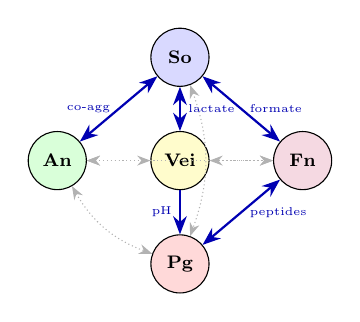
\begin{tikzpicture}[scale=0.82, every node/.style={transform shape},
    species/.style={circle, draw, minimum size=0.9cm, font=\footnotesize\bfseries},
    edge/.style={<->, thick, >=Stealth},
    uniedge/.style={->, thick, blue!70!black, >=Stealth},
    weakedge/.style={<->, thin, gray!60, >=Stealth, densely dotted}
]
    \node[species, fill=blue!15] (so) at (0, 2.2) {So};
    \node[species, fill=green!15] (an) at (-1.9, 0.6) {An};
    \node[species, fill=yellow!20] (vei) at (0, 0.6) {Vei};
    \node[species, fill=purple!15] (fn) at (1.9, 0.6) {Fn};
    \node[species, fill=red!15] (pg) at (0, -1.0) {Pg};
    \draw[edge, blue!70!black] (so) -- (an) node[midway, left, font=\tiny] {co-agg};
    \draw[edge, blue!70!black] (so) -- (vei) node[midway, right, font=\tiny] {lactate};
    \draw[edge, blue!70!black] (so) -- (fn) node[midway, right, font=\tiny] {formate};
    \draw[uniedge] (vei) -- (pg) node[midway, left, font=\tiny] {pH};
    \draw[edge, blue!70!black] (fn) -- (pg) node[midway, right, font=\tiny] {peptides};
    \draw[weakedge] (an) -- (vei);
    \draw[weakedge] (an) -- (fn);
    \draw[weakedge] (vei) -- (fn);
    \draw[weakedge] (so) to[bend left=20] (pg);
    \draw[weakedge] (an) to[bend right=20] (pg);
\end{tikzpicture}
\end{minipage}%
\hfill
\begin{minipage}[t]{0.65\textwidth}
\vspace{0pt}
\small
\begin{tabular}{@{}lll@{}}
\toprule
\textbf{Pair} & \textbf{Mechanism} & \textbf{Reported flow}\\
\midrule
So--An & Co-aggregation & mutual\\
So--Vei & Lactate exchange & So to Vei\\
So--Fn & Formate symbiosis & mutual\\
Vei--Pg & pH elevation & Vei to Pg\\
Fn--Pg & Peptide supply & mutual\\
\bottomrule
\end{tabular}
\captionof{table}{Previously reported or biologically supported interactions~\citep{heine2025influence} used to interpret the inferred coefficients. The model coefficients $a_{ij}$ are symmetric; the last column refers to the reported metabolite flow, not to the model. All 15 parameters are estimated; none is fixed a priori.}
\label{tab:active}
\end{minipage}
\caption{Species interaction network~\citep{heine2025influence}. Solid: previously reported or biologically supported interactions considered in the interpretation of the model. Dotted grey: no reported pathway. All pairs are estimated with the same prior.}
\label{fig:network}
\end{figure}

\section{Likelihood weights and algorithm}
\label{sec:S_alg}
\begin{table}[htbp]\centering\small
\begin{tabular}{@{}lll@{}}\toprule
Weight & Value & Applies to\\\midrule
$\lambda_{\mathrm{Pg}}$ & 5 & Pg, all time points\\
$\lambda_{\mathrm{late}}$ & 3 & Days 15 and 21, all species\\
$\lambda_{\mathrm{rare}}$ & 0.1 & species with mean fraction $<5\%$\\
$\lambda_{\psi}$ & 3.0 (DH), 2.0 (DS), 1.5 (CS, CH) & viability channel, Phase~2\\\bottomrule
\end{tabular}
\caption{Likelihood weights.}
\label{tab:weights}
\end{table}

\begin{algorithm}[t]
\caption{Staged GPU-accelerated TMCMC (one seed; every stage is run with three seeds and checked as in the main text)}
\label{alg:tmcmc}
\begin{algorithmic}[1]
\REQUIRE Composition data $\yobs$, viability data, $N_p$ particles, GPU device
\ENSURE MAP estimate $\hat{\btheta}^{\mathrm{MAP}}$, posterior samples, log-evidence $\ln\hat{Z}$
\STATE $\triangleright$ \textbf{Stage (i): composition likelihood, initial box}
\STATE Draw $\{\btheta_j\}_{j=1}^{N_p}$ from the stage prior; set $\beta_0\leftarrow 0$
\WHILE{$\beta_m < 1$}
    \STATE Find $\beta_{m+1}$ s.t.\ $\mathrm{CoV}[\{w_j\}]=\delta_{\mathrm{target}}$ via bisection
    \STATE Compute weights $w_j \leftarrow p(\yobs\mid\btheta_j)^{\beta_{m+1}-\beta_m}$
    \STATE Resample $N_p$ particles $\propto w_j$ (systematic)
    \STATE Estimate weighted covariance $\hat{\boldsymbol{\Sigma}}^{(m)}$ (weighted particle covariance)
    \FOR{$k = 1$ \TO $K$}
        \STATE Propose $\btheta_{j}'$ for all $j$ (random-walk or differential-evolution move)
        \STATE Evaluate all $N_p$ likelihoods in parallel via \texttt{jax.vmap} on GPU
        \STATE Accept/reject via MH ; reject proposals outside the box
    \ENDFOR
\ENDWHILE
\STATE Record MAP and posterior SD per parameter
\STATE $\triangleright$ \textbf{Stage (ii): composition likelihood, box mean $\pm4$\,SD}
\STATE Repeat lines 2--13 on the narrowed box, starting from the previous particles
\STATE $\triangleright$ \textbf{Stages (iii)--(iv): add the viability channel; initial box, then mean $\pm4$\,SD}
\STATE Augment likelihood with the weighted viability channel (Table~\ref{tab:weights})
\STATE Repeat lines 2--13 for each stage
\RETURN $\hat{\btheta}^{\mathrm{MAP}}$, posterior samples, $\ln\hat{Z}$
\end{algorithmic}
\end{algorithm}

\begin{table}[htbp]
\centering\small
\begin{tabular}{@{}lrrr@{}}
\toprule
\textbf{Metric} & \textbf{CPU (12 cores)} & \textbf{GPU (RTX\,4090)} & \textbf{Speedup}\\
\midrule
\multicolumn{4}{@{}l}{\textit{Matched benchmark (DH, $N_p=500$, $K=10$, 9 stages):}}\\
\quad Per stage     & 2\,400\,s   & 14\,s    & $170\times$\\
\quad Total         & 21\,600\,s  & 147\,s   & $\mathbf{147\times}$\\
\midrule
\multicolumn{4}{@{}l}{\textit{Final stage (iv) (4 cond., $N_p=\TBD{n}$, $K=\TBD{n}$, GPU \TBD{model}):}}\\
\numTimingRows
\bottomrule
\end{tabular}
\caption{Computational cost comparison.
The matched benchmark (500 particles, identical settings) isolates the GPU speedup at about 150--170$\times$ (170$\times$ per stage, 147$\times$ in total).
The final-stage times are measured per seed \TBD{update with the final runs}.
$^\dagger$Extrapolated from the 500-particle CPU benchmark assuming linear scaling in~$N_p$.}
\label{tab:timing}
\end{table}

\section{Prior boxes}
\label{sec:S_boxes}
Table~\ref{tab:S_boxes} lists the uniform prior box of every interaction entry for each condition and stage.
The initial box was set empirically to contain earlier posterior estimates and encodes no sign constraint.
An entry was widened only where more than 20\% of its posterior mass lay in the outer 5\% of the range on one side, or where this fraction increased by more than 0.10 between stages with the same likelihood; the stage was then repeated.
The last column gives $\ln V=\sum_k\ln(u_k-l_k)$, the log-volume of the box, which enters $\ln\hat Z$ and is the reason why $\ln\hat Z$ is not compared across conditions.

\begin{table}[h]
\centering
\caption{Prior boxes per condition and stage for the 15 free entries; entries widened relative to stage (i) in bold. Stage (iv) uses the stage-(iii) posterior mean $\pm4$\,SD, clipped to the stage-(iii) box. $\ln V=\sum_k\ln(u_k-l_k)$ over the free entries.}
\label{tab:S_boxes}
\small% placeholder: run tools/make_supplementary_tables.py
\multicolumn{5}{l}{\TBD{run tools/make\_supplementary\_tables.py}}\\

\end{table}

\section{Runs and convergence}
\label{sec:S_runs}
Table~\ref{tab:S_runs} lists, for every condition and stage, the number of particles and mutation steps, the number of tempering stages, the acceptance rate, the moves per parameter, and the spread over the three seeds of the maximum log-likelihood and of the posterior medians (criteria (i)--(iv) of the main text).

\begin{table}[h]
\centering
\caption{Runs of the final pipeline: particles $N_p$, mutation steps $K$, tempering stages, acceptance rate, moves per free parameter, maximum log-likelihood (best seed; spread over three seeds in parentheses) and wall-clock hours per seed.}
\label{tab:S_runs}
\small% placeholder: run tools/make_supplementary_tables.py
\multicolumn{9}{l}{\TBD{run tools/make\_supplementary\_tables.py}}\\

\end{table}

\section{Identifiability of the interaction entries}
\label{sec:S_ident}
Table~\ref{tab:S_ident} lists, for the final stage (iv) of every condition, the median and the 90\% interval of each entry, pooled over the three seeds.
An entry whose posterior standard deviation is at least 0.8 times that of a uniform distribution on its box is shown in grey and excluded from the seed-agreement criterion: the data do not constrain its magnitude beyond the prior box. Among these, entries whose 90\% interval excludes zero are marked s.o. (sign only), the others n.i. (not identified).

\begin{table}[h]
\centering
\caption{Posterior median [5\%, 95\%] of the 15 entries at stage (iv), three seeds pooled. Grey: the posterior spreads over most of the box (standard deviation $\ge0.8$ times that of a uniform distribution on the box); n.i.: not identified, s.o.: sign only (the 90\% interval excludes zero).}
\label{tab:S_ident}
\small% placeholder: run tools/make_supplementary_tables.py
\begin{tabular}{lcccc}\toprule
\multicolumn{5}{l}{\TBD{run tools/make\_supplementary\_tables.py}}\\
\bottomrule\end{tabular}

\end{table}

\section{Bayes factor for the \textit{Fn}--\textit{Pg} interaction}
\label{sec:S_bayes}
Stage~(i) was repeated with $a_{45}=0$ for all four conditions (three seeds each).
Table~\ref{tab:S_bayes} reports $\ln\hat Z$ of both models, $\ln B=\ln\hat Z_{\mathrm{full}}-\ln\hat Z_{a_{45}=0}$, and the width of the $a_{45}$ box, which sets the Occam penalty.

\begin{table}[h]
\centering
\caption{Log-evidence of the full and the reduced ($a_{45}=0$) model at stage (i), mean $\pm$ half-range over three seeds, and $\ln B=\ln\hat Z_{\mathrm{full}}-\ln\hat Z_{a_{45}=0}$. The last two columns give the $a_{45}$ box and its log-width, which enters $\ln\hat Z_{\mathrm{full}}$ as an Occam penalty.}
\label{tab:S_bayes}
\small% placeholder: run tools/make_supplementary_tables.py
\multicolumn{6}{l}{\TBD{run tools/make\_supplementary\_tables.py}}\\

\end{table}

\paragraph{Dysbiotic Static.}
In DS, $a_{45}$ and $a_{33}$ trade off. With $a_{45}=0$ the posterior moves almost entirely to the mode $a_{33}\approx-10$ (weight \TBD{0.83--0.87}), whereas the full model places most of its mass at $a_{33}\approx+1$ (weight of the mode $a_{33}<-5$: \TBD{0.09--0.12}).
Table~\ref{tab:S_modes} gives $a_{45}$ separately for each mode.

\begin{table}[h]
\centering
\caption{DS: $a_{45}$ by $a_{33}$ mode (stage \TBD{iv}, three seeds).}
\label{tab:S_modes}
\begin{tabular}{lccc}
\toprule
Mode & Particles & $a_{45}$ median [5\%, 95\%] & max log-likelihood\\
\midrule
$a_{33}\ge-5$ & \TBD{} & \TBD{+2.4 [+0.5, +4.4]} & \TBD{}\\
$a_{33}<-5$   & \TBD{} & \TBD{+0.8 [$-$0.2, +1.4]} & \TBD{}\\
\bottomrule
\end{tabular}
\end{table}

\section{Likelihood weights}
\label{sec:S_lambda}
Stage~(i) for DH was repeated with $\lambda_{\mathrm{Pg}}=\lambda_{\mathrm{late}}=1$ (1000 particles, 100 mutation steps, three seeds; all convergence criteria met). Table~\ref{tab:S_lambda} compares it with the weighted run.

\begin{table}[h]
\centering
\caption{DH, stage (i): weighted ($\lambda_{\mathrm{Pg}}=5$, $\lambda_{\mathrm{late}}=3$) and unweighted likelihood. Ranges over three seeds.}
\label{tab:S_lambda}
\begin{tabular}{lccc}
\toprule
 & $a_{45}$ median [5\%, 95\%] & Pg D21/D15 (measured 2.74) & RMSE\\
\midrule
Weighted   & $+2.9$ to $+3.2$ [$+0.5$ to $+1.1$, $+5.2$ to $+5.5$] & 2.4--2.9 & 0.058--0.065\\
Unweighted & $+3.0$ [$-0.06$ to $+0.17$, $+5.6$] & 1.7--3.1 & 0.059--0.068\\
\bottomrule
\end{tabular}
\end{table}

\bibliographystyle{elsarticle-harv}
\bibliography{references_ikm}
\end{document}
